\documentclass[11pt,a4paper]{article}
\usepackage[utf8]{inputenc}
\usepackage[T1]{fontenc}
\usepackage[spanish,es-noquoting]{babel}
\usepackage{lmodern,microtype}
\usepackage[margin=1.65cm,top=1.55cm,bottom=1.55cm]{geometry}
\usepackage{graphicx,booktabs,array,longtable,tabularx,ragged2e}
\usepackage{xcolor,hyperref,fancyhdr,enumitem,multicol,caption}
\usepackage{float}
\hypersetup{colorlinks=true,linkcolor=black,citecolor=black,urlcolor=blue!50!black}
\definecolor{verde}{HTML}{1F644C}
\definecolor{gris}{HTML}{57616B}
\renewcommand{\arraystretch}{1.12}
\setlength{\parskip}{3pt}
\setlength{\parindent}{0pt}
\setlength{\tabcolsep}{3.2pt}
\captionsetup{font=footnotesize,labelfont=bf}
\pagestyle{fancy}\fancyhf{}
\fancyhead[L]{\footnotesize UTEQ \quad ISR-401 \quad TA-IND-01}
\fancyhead[R]{\footnotesize Análisis de Facebook en Android 16}
\fancyfoot[C]{\footnotesize Página \thepage}
\renewcommand{\headrulewidth}{0.35pt}
\newcommand{\seccion}[1]{\par\vspace{6pt}\noindent{\color{verde}\large\bfseries #1}\par\vspace{4pt}}
\newcommand{\ft}[1]{\textcolor{verde}{\textbf{#1}}}
\begin{document}
{\color{verde}\Large\bfseries Ingeniería de requisitos en una aplicación conocida: Facebook}\par
\vspace{3pt}
{\small\textbf{Estudiante:} FUERTES CALVO LANDY LORENA \quad\textbf{Asignatura:} Ingeniería de Requerimientos (ISR-401)}\par
{\small\textbf{Actividad:} TA-IND-01 \quad\textbf{Fecha de elaboración:} 11 de noviembre de 2026 \quad\textbf{Equipo:} Samsung, Android 16}\par
\vspace{4pt}\hrule\vspace{5pt}
\seccion{1. Sistema elegido y alcance de la observación}
Facebook es una red social que permite consultar publicaciones, crear contenido, reaccionar a publicaciones y gestionar interacciones entre cuentas. En este análisis se considera la versión móvil utilizada en un dispositivo Samsung con Android 16. Los usuarios principales son personas que consultan contenidos y se comunican con otras cuentas; entre los interesados también se encuentran quienes administran la plataforma. Se observaron seis pantallas: Inicio, Nueva publicación, Reacciones, Buscar, Notificaciones y Cuenta de Meta. Las capturas documentan elementos de interfaz, no el funcionamiento de los servidores ni el cumplimiento de objetivos de rendimiento o seguridad. Las pruebas y umbrales posteriores son propuestas para una especificación académica, no mediciones ya ejecutadas.
\seccion{2. Resumen analítico de ISO/IEC/IEEE 29148:2018}
La ingeniería de requisitos no consiste únicamente en listar funciones de una aplicación: transforma necesidades de usuarios e interesados en especificaciones que puedan discutirse, implementarse y comprobarse. La cláusula 1 sitúa esta actividad dentro del ciclo de vida de sistemas y software. En Facebook, observar un botón no constituye por sí solo un requisito; es necesario señalar qué necesidad cubre, qué respuesta se espera y bajo cuáles circunstancias. La cláusula 5.2.3 permite entender la diferencia entre una intención inicial, como «quiero localizar publicaciones», y una obligación delimitada, como presentar entradas de la sección Recientes cuando exista historial de búsqueda. Las capturas sirven de evidencia de interfaz, pero no permiten conocer decisiones internas de Meta \cite{ISO29148}.

Para construir un requisito bien formado, la cláusula 5.2.4 indica que debe expresarse una capacidad, propiedad o restricción atribuible al sistema, con condiciones claras y posibilidad de comprobación. Por ello se adopta un sujeto explícito («la aplicación Facebook»), una obligación concreta y un resultado observable. Por ejemplo, se precisa que la persona tiene una sesión iniciada o que el historial contiene entradas; de otro modo, podría exigirse mostrar información inexistente. El análisis diferencia la capacidad del sistema de la habilidad de quien lo utiliza: un requisito funcional señala qué presentará el producto tras una acción, mientras que la facilidad de localización de un control requeriría una prueba de uso con una población y un contexto definidos. Esto evita confundir una función visible con su nivel de calidad \cite{ISO29148}.

La cláusula 5.2.5 identifica \textbf{nueve características de un requisito individual}. Debe ser \emph{necesario}, porque su ausencia dejaría una necesidad sin atender, y \emph{apropiado}, porque su nivel de detalle debe corresponder al alcance sin imponer soluciones técnicas superfluas. Debe ser \emph{no ambiguo}, es decir, admitir una interpretación definida; \emph{completo}, de modo que las condiciones y el resultado puedan entenderse sin información pendiente; y \emph{singular}, porque cada enunciado ha de expresar una obligación principal. Separar el listado de avisos (RF-05), los botones de una solicitud (RI-07) y la ausencia de cierres inesperados (RC-14) evita evaluar tres obligaciones como si fueran una sola. A su vez, un requisito singular puede incorporar varias condiciones previas siempre que no mezcle resultados independientes. La singularidad es importante durante la aceptación: cuando una prueba falla, debe ser posible identificar qué obligación concreta se incumplió sin declarar fallido un conjunto de comportamientos diferentes \cite{ISO29148}.

Las otras cuatro características son \emph{factible}, \emph{verificable}, \emph{correcto} y \emph{conforme}. La factibilidad considera limitaciones técnicas, económicas y del entorno; la verificabilidad implica disponer de una forma objetiva de inspeccionar, demostrar, analizar o probar el cumplimiento. La corrección significa reflejar la necesidad que originó el requisito, mientras que la conformidad exige respetar las reglas y el formato acordados. La frase «Facebook debe cargar rápido» no establece una prueba objetiva; «mostrar la primera publicación en tres segundos o menos bajo condiciones definidas» sí permite diseñarla. Ese tiempo es un \emph{umbral propuesto}, no una medición del producto \cite{ISO29148}.

La cláusula 5.2.6 traslada la evaluación al \textbf{conjunto de requisitos}. No basta con que cada uno esté bien redactado: el conjunto ha de ser \emph{completo}, \emph{consistente}, \emph{factible}, \emph{comprensible} y \emph{susceptible de validación}. Completo significa cubrir las necesidades del alcance delimitado; aquí se analizan seis pantallas y no toda la plataforma. Consistente implica evitar contradicciones, duplicidades y cambios de terminología: los controles «Confirmar» y «Eliminar» deben conservar esos nombres en RI-07 y RH-10. Factible requiere que las obligaciones puedan coexistir dentro de las restricciones del entorno, no solo que cada una sea posible por separado. Comprensible exige una organización interpretable por los interesados, y validable supone que pueda determinarse si el conjunto satisface las necesidades que le dieron origen. La falta de acceso a la arquitectura y a interesados oficiales limita esa validación. Por ejemplo, una pantalla puede incluir el control «Confirmar», pero la especificación quedaría incompleta para un uso profesional si no se consideraran también los escenarios de error, permisos y estados vacíos. La consistencia debe revisarse entre requisitos, no solo dentro de cada oración: si un enunciado exigiera permitir el acceso a datos tras cerrar sesión y otro lo prohibiera, las dos obligaciones no podrían aceptarse simultáneamente. En este trabajo se reconoce ese límite de alcance en lugar de afirmar una completitud no demostrada \cite{ISO29148}.

La cláusula 5.2.7 aborda el \textbf{lenguaje de los requisitos}. Valoraciones como «fácil», «intuitivo» o «cómodo» dependen de apreciaciones personales; adverbios como «rápido» y «al instante» carecen de magnitud y unidad. Superlativos como «el mejor» y comparaciones como «más seguro» necesitan una referencia comprobable. «Y/o» puede ocultar si debe cumplirse una condición, la otra o ambas. Los absolutos «siempre», «todos» o «nunca» resultan problemáticos cuando no se delimitan los escenarios. También conviene evitar pronombres sin antecedente, «entre otros», «si es posible» y referencias a documentos sin versión precisa. En los requisitos de Facebook se sustituyen estas expresiones por condiciones acotadas (sesión válida o Wi-Fi de al menos 20 Mb/s), unidades (segundos y dp) y muestras finitas (19 de 20 aperturas o 30 intentos), sin presentar dichas cifras como pruebas ejecutadas. La formulación original «el buscador funcionará siempre» no permite enumerar las situaciones que supuestamente cubre; en cambio, «mostrar una entrada de Recientes cuando exista historial» delimita el escenario y deja planteado un resultado inspeccionable. Similarmente, «botones cómodos» se sustituye por una dimensión táctil expresada en dp. Especificar la medida no demuestra que la aplicación ya cumpla ese objetivo: únicamente vuelve comprobable la propuesta \cite{ISO29148}.

La cláusula 5.2.8 distingue los \textbf{atributos} de los \textbf{tipos de requisitos}. El apartado 5.2.8.1 presenta la idea general de atributos y 5.2.8.2 ofrece ejemplos: identificador, origen, prioridad, justificación y otros datos de gestión que facilitan administrar y rastrear requisitos sin sustituir su enunciado. Por ejemplo, RF-04 identifica una obligación funcional ligada a la captura F4 y a un criterio de aceptación. El \emph{tipo}, desarrollado en 5.2.8.3, indica la naturaleza de la obligación: funcional (abrir el editor, RF-02), de interfaz (botones, RI-07), de proceso (documentar pruebas antes de una versión, RP-08), de usabilidad/calidad en uso (localizar Buscar, RU-09), de factores humanos (área táctil, RH-10) o de calidad del producto (RC-11 a RC-15). La distinción evita usar la palabra «atributo» como si fuera sinónimo de «no funcional»: el identificador y el origen sirven para administrar el requisito, mientras que un tiempo de respuesta máximo es parte del comportamiento exigido. Los requisitos de proceso, por su parte, describen actividades esperadas del equipo de desarrollo; una captura no demuestra que esas actividades se ejecuten realmente, por lo que RP-08 se plantea explícitamente como una regla hipotética \cite{ISO29148}.

Para estos cinco últimos se utiliza ISO/IEC 25010:2023, que clasifica la calidad por características y subcaracterísticas; entre las aplicadas figuran eficiencia de desempeño, capacidad de interacción, fiabilidad y seguridad \cite{ISO25010}. SWEBOK v4.0 complementa el enfoque de especificación y verificación \cite{SWEBOK4}. Conviene separar \emph{verificación} de la redacción (cláusula 3.1.26) y \emph{validación} respecto a la necesidad del interesado (3.1.25): una oración puede ser técnicamente comprobable y aun así describir una función que no resuelve el problema de usuario. Por eso las seis capturas respaldan controles visibles, mientras que los umbrales representan criterios de aceptación pendientes de ejecución \cite{ISO29148}.

\seccion{3. Glosario de la cláusula 3}
Las definiciones siguientes son paráfrasis situadas en el contexto observado, no transcripciones de la norma \cite{ISO29148}.
\vspace{3pt}\footnotesize
\begin{longtable}{@{}p{3.3cm}p{5.6cm}p{7.9cm}@{}}\toprule
\textbf{Término y cláusula}&\textbf{Definición propia}&\textbf{Ejemplo en Facebook}\\\midrule\endhead
Atributo (3.1.2) & Propiedad de un elemento que puede distinguirse o medirse. & El tiempo de carga de Inicio se expresa en segundos.\\\addlinespace[2pt]
Condición (3.1.6) & Circunstancia comprobable en la que aplica una obligación. & Buscar muestra Recientes cuando existe una consulta registrada.\\\addlinespace[2pt]
Restricción (3.1.7) & Límite externo impuesto al sistema o a su desarrollo. & Una restricción normativa propuesta es que el tratamiento de datos personales cumpla la legislación aplicable.\\\addlinespace[2pt]
Requisito (3.1.19) & Expresión precisa de una necesidad del sistema. & Se solicita mostrar la pantalla Nueva publicación al tocar el editor.\\\addlinespace[2pt]
Elicitación (3.1.20) & Obtención sistemática de necesidades de usuarios e interesados. & En una entrevista propuesta, preguntar a usuarios qué dificultades encuentran al buscar publicaciones.\\\addlinespace[2pt]
Ingeniería de requisitos (3.1.21) & Trabajo de definir, analizar, validar y mantener obligaciones del producto. & Refinar un pedido informal sobre reacciones hasta hacerlo comprobable.\\\addlinespace[2pt]
Trazabilidad (3.1.23) & Relación documentada entre una necesidad y sus especificaciones o pruebas. & La necesidad de localizar contenido se vincula con RF-04 y con su criterio de aceptación.\\\addlinespace[2pt]
Validación de requisitos (3.1.25) & Revisión de si lo especificado responde a la necesidad real. & Consultar si ver Recientes ayuda al usuario a repetir una búsqueda.\\\addlinespace[2pt]
Verificación de requisitos (3.1.26) & Revisión de si los enunciados están correctamente escritos. & Comprobar que RC-11 define condición, unidad y umbral.\\\addlinespace[2pt]
Interesado (3.1.28) & Persona u organización afectada o interesada en las propiedades del sistema. & Quien recibe solicitudes de amistad es interesado de Notificaciones.\\\addlinespace[2pt]
\bottomrule\end{longtable}\normalsize
\seccion{4. Requisitos propuestos y clasificación}
La tabla agrupa quince requisitos de seis tipos. \textbf{F1--F6} identifican las pantallas aportadas como evidencia. Los objetivos de calidad RC-11 a RC-15 son \emph{umbrales propuestos y no resultados comprobados}; RU-09, RH-10 y RP-08 también necesitan actividades posteriores para su comprobación. Un criterio de aceptación define qué se revisaría, no equivale a afirmar que la prueba fue ejecutada \cite{ISO29148,ISO25010}. Los límites de 3 s, 2 s y 19/20 aperturas (95\%) se proponen como objetivos didácticos, sujetos a validación con interesados; no son metas oficiales de Meta. Para RH-10 se adopta 48 $\times$ 48 dp como referencia de accesibilidad publicada para interfaces Android \cite{AndroidAcc}.
{\scriptsize\setlength{\tabcolsep}{2.3pt}
\begin{longtable}{@{}p{1.0cm}p{7.0cm}>{\RaggedRight\arraybackslash}p{1.65cm}>{\RaggedRight\arraybackslash}p{3.3cm}>{\RaggedRight\arraybackslash}p{3.55cm}@{}}
\caption{Quince requisitos, clasificación, métrica y aceptación.}\label{tab:requisitos}\\
\toprule \textbf{ID} & \textbf{Enunciado final de requisito} & \textbf{Tipo / F} & \textbf{ISO/IEC 25010:2023, si aplica} & \textbf{Métrica y criterio de aceptación}\\\midrule\endfirsthead
\multicolumn{5}{l}{\emph{Tabla \thetable\ (continuación)}}\\\toprule
\textbf{ID} & \textbf{Enunciado final de requisito} & \textbf{Tipo / F} & \textbf{ISO 25010 (si aplica)} & \textbf{Métrica y aceptación}\\\midrule\endhead
\textbf{RF-01} & Al acceder a Inicio con una sesión válida y contenido disponible, la aplicación Facebook mostrará al menos una tarjeta de publicación en el área central. & Func. / F1 & No aplica & Presencia de tarjeta: 1 tarjeta visible en inicio cuando exista contenido\\\addlinespace[3pt]
\textbf{RF-02} & Al seleccionar «¿Qué estás pensando?» en Inicio, la aplicación Facebook abrirá un editor de nueva publicación con un campo para introducir texto. & Func. / F2 & No aplica & Apertura del editor: 1 editor visible al seleccionar el cuadro de publicación\\\addlinespace[3pt]
\textbf{RF-03} & Al abrir el selector de reacciones de una publicación, la aplicación Facebook presentará al menos dos opciones de reacción diferenciables. & Func. / F3 & No aplica & Opciones de reacción: El selector presenta al menos 2 reacciones distintas\\\addlinespace[3pt]
\textbf{RF-04} & Al abrir Buscar con al menos una consulta reciente registrada, la aplicación Facebook mostrará una entrada en la sección «Recientes». & Func. / F4 & No aplica & Entradas recientes visibles: 1 entrada reciente cuando exista historial\\\addlinespace[3pt]
\textbf{RF-05} & Al acceder a Notificaciones con avisos disponibles, la aplicación Facebook mostrará al menos un elemento en el listado de notificaciones. & Func. / F5 & No aplica & Listado de avisos: 1 notificación visible cuando existan notificaciones\\\addlinespace[3pt]
\textbf{RF-06} & Al abrir Cuenta de Meta, la aplicación Facebook presentará una opción identificada como «Inicio de sesión y seguridad». & Func. / F6 & No aplica & Opción de seguridad: 1 opción «Inicio de sesión y seguridad» visible\\\addlinespace[3pt]
\textbf{RI-07} & En la tarjeta de una solicitud de amistad recibida, la interfaz de Facebook mostrará dos controles diferenciados con las etiquetas «Confirmar» y «Eliminar». & Interfaz / F5 & No aplica & Acciones diferenciadas: Botones «Confirmar» y «Eliminar» distinguibles\\\addlinespace[3pt]
\textbf{RP-08} & Como regla de proceso propuesta, antes de liberar una versión que modifique las solicitudes de amistad, el equipo responsable registrará el resultado de diez casos de prueba de aceptación asociados a esa función. & Proceso / F5 & No aplica & Registro de casos: 10 casos documentados antes de cada entrega que afecte solicitudes\\\addlinespace[3pt]
\textbf{RU-09} & En una prueba propuesta con cinco usuarios sin experiencia previa en Facebook, al menos cuatro localizarán el acceso a Buscar en un máximo de veinte segundos sin ayuda. & Uso / F4 & No aplica & Usuarios que identifican Buscar: $\geq$4/5 usuarios en $\leq$20 s sin ayuda\\\addlinespace[3pt]
\textbf{RH-10} & Como requisito propuesto para la pantalla Notificaciones de Android, cada control «Confirmar» y «Eliminar» tendrá un área táctil de al menos 48 $\times$ 48 dp. & Factor humano / F5 & No aplica & Área táctil mínima: 48 $\times$ 48 dp para cada control\\\addlinespace[3pt]
\textbf{RC-11} & Con una conexión Wi-Fi de al menos 20 Mb/s y sesión iniciada en Samsung Android 16, la pantalla Inicio mostrará su primera publicación en tres segundos o menos en al menos diecinueve de veinte aperturas. & Calidad / F1 & Eficiencia de desempeño / Comportamiento temporal & Tiempo de carga de Inicio: $\leq$3 s en $\geq$19/20 aperturas con Wi-Fi $\geq$20 Mb/s\\\addlinespace[3pt]
\textbf{RC-12} & Con una conexión Wi-Fi de al menos 20 Mb/s y una entrada guardada en el historial, la pantalla Buscar mostrará la sección Recientes en dos segundos o menos en al menos diecinueve de veinte aperturas. & Calidad / F4 & Eficiencia de desempeño / Comportamiento temporal & Tiempo para lista Recientes: $\leq$2 s en $\geq$19/20 aperturas con Wi-Fi $\geq$20 Mb/s\\\addlinespace[3pt]
\textbf{RC-13} & Con el editor de una publicación vacío, el control «Siguiente» permanecerá inactivo en los veinte intentos consecutivos de avanzar sin ingresar contenido. & Calidad / F2 & Capacidad de interacción / Protección contra errores del usuario & Bloqueo con editor vacío: 20/20 intentos sin avanzar con editor vacío\\\addlinespace[3pt]
\textbf{RC-14} & Durante treinta aperturas consecutivas de Notificaciones en Samsung Android 16, la aplicación Facebook registrará cero cierres inesperados. & Calidad / F5 & Fiabilidad / Ausencia de fallos & Cierres inesperados: 0 cierres en 30 aperturas de Notificaciones\\\addlinespace[3pt]
\textbf{RC-15} & Tras cerrar sesión, la aplicación Facebook exigirá nueva autenticación antes de mostrar información de la cuenta en «Tu información y permisos», en 20 intentos consecutivos de acceso. & Calidad / F6 & Seguridad / Confidencialidad & Acceso sin autenticación: 0 accesos privados en 20 intentos tras cierre de sesión\\\addlinespace[3pt]
\bottomrule\end{longtable}}
\seccion{5. Autoevaluación de los quince requisitos}
La tabla presenta una revisión preliminar de borradores ilustrativos frente a las nueve características de la cláusula 5.2.5: \textbf{N} necesario, \textbf{A} apropiado, \textbf{U} unívoco, \textbf{C} completo, \textbf{S} singular, \textbf{F} factible, \textbf{V} verificable, \textbf{R} correcto y \textbf{Co} conforme. En la matriz, \textbf{1} indica criterio satisfecho en la revisión de redacción y \textbf{0} indica aspecto que motivó corrección. \emph{Factibilidad y corrección se consideran provisionales}, pues no se dispone de acceso al equipo de desarrollo ni de validación formal con interesados.
{\footnotesize\centering
\begin{tabular}{@{}l*{9}{c}p{5.8cm}@{}}\toprule
\textbf{ID}&\textbf{N}&\textbf{A}&\textbf{U}&\textbf{C}&\textbf{S}&\textbf{F}&\textbf{V}&\textbf{R}&\textbf{Co}&\textbf{Defecto principal del borrador}\\\midrule
RF-01 & 1 & 1 & 0 & 0 & 1 & 1 & 0 & 1 & 0 & Ambiguo; actor y condición ausentes.\\
RF-02 & 1 & 0 & 0 & 0 & 1 & 1 & 0 & 1 & 0 & Lenguaje subjetivo y acción no definida.\\
RF-03 & 1 & 1 & 0 & 0 & 1 & 1 & 0 & 0 & 0 & Superlativo y cantidad imprecisa.\\
RF-04 & 1 & 1 & 0 & 0 & 1 & 0 & 0 & 1 & 0 & Totalidad no demostrable y falta condición.\\
RF-05 & 1 & 1 & 0 & 0 & 1 & 0 & 0 & 1 & 0 & «Siempre» es absoluto y no fija contexto.\\
RF-06 & 1 & 0 & 0 & 0 & 1 & 1 & 0 & 1 & 0 & Acción genérica y subjetiva.\\
RI-07 & 1 & 1 & 0 & 0 & 0 & 1 & 0 & 1 & 0 & Valoración estética; no define controles.\\
RP-08 & 1 & 1 & 0 & 0 & 1 & 0 & 0 & 0 & 0 & Cantidad y momento sin precisar.\\
RU-09 & 1 & 1 & 0 & 0 & 1 & 1 & 0 & 1 & 0 & «Muy fácil» es subjetivo.\\
RH-10 & 1 & 1 & 0 & 0 & 1 & 0 & 0 & 1 & 0 & Comparación subjetiva sin unidad.\\
RC-11 & 1 & 1 & 0 & 0 & 1 & 0 & 0 & 1 & 0 & Adverbio sin medición.\\
RC-12 & 1 & 1 & 0 & 0 & 1 & 0 & 0 & 1 & 0 & Absoluto y tiempo indeterminado.\\
RC-13 & 1 & 1 & 0 & 0 & 1 & 1 & 0 & 1 & 0 & Error no definido ni verificable.\\
RC-14 & 1 & 1 & 0 & 0 & 1 & 1 & 0 & 0 & 0 & Expresión absoluta, sin alcance.\\
RC-15 & 1 & 1 & 0 & 0 & 0 & 0 & 0 & 1 & 0 & Totalidad y noción de protección genérica.\\
\bottomrule\end{tabular}}
\par\smallskip
Las versiones corregidas propuestas eliminan términos ambiguos, precisan condiciones y aportan criterios de aceptación (Tabla~\ref{tab:requisitos}). Por ejemplo, en RC-11 se marca U=0 porque «súper rápido» es subjetivo, C=0 por omitir condiciones de red y V=0 porque no fija un límite medible. La corrección añade conexión, tres segundos y 19/20 aperturas. La matriz califica versiones \emph{anteriores}; no es una prueba del producto ni valida automáticamente la pertinencia de todos los requisitos.
{\scriptsize\setlength{\tabcolsep}{3pt}
\begin{longtable}{@{}p{1.0cm}p{5.4cm}p{9.8cm}@{}}
\caption{Versión inicial y versión corregida de cada requisito.}\label{tab:correccion}\\
\toprule\textbf{ID}&\textbf{Enunciado anterior (por corregir)}&\textbf{Enunciado corregido}\\\midrule\endfirsthead
\multicolumn{3}{l}{\emph{Tabla \thetable\ (continuación)}}\\\toprule
\textbf{ID}&\textbf{Anterior}&\textbf{Corregido}\\\midrule\endhead
\textbf{RF-01} & El inicio de la aplicación tiene que mostrar publicaciones variadas. & Al acceder a Inicio con una sesión válida y contenido disponible, la aplicación Facebook mostrará al menos una tarjeta de publicación en el área central.\\\addlinespace[2.5pt]
\textbf{RF-02} & El usuario podrá crear un post fácilmente desde la pantalla de inicio. & Al seleccionar «¿Qué estás pensando?» en Inicio, la aplicación Facebook abrirá un editor de nueva publicación con un campo para introducir texto.\\\addlinespace[2.5pt]
\textbf{RF-03} & Las publicaciones tendrán las mejores reacciones disponibles para elegir. & Al abrir el selector de reacciones de una publicación, la aplicación Facebook presentará al menos dos opciones de reacción diferenciables.\\\addlinespace[2.5pt]
\textbf{RF-04} & El buscador mostrará siempre todo lo que se buscó antes en la cuenta. & Al abrir Buscar con al menos una consulta reciente registrada, la aplicación Facebook mostrará una entrada en la sección «Recientes».\\\addlinespace[2.5pt]
\textbf{RF-05} & En la pestaña de notificaciones siempre saldrán los avisos del usuario. & Al acceder a Notificaciones con avisos disponibles, la aplicación Facebook mostrará al menos un elemento en el listado de notificaciones.\\\addlinespace[2.5pt]
\textbf{RF-06} & La aplicación dará opciones para configurar bien la seguridad de la cuenta. & Al abrir Cuenta de Meta, la aplicación Facebook presentará una opción identificada como «Inicio de sesión y seguridad».\\\addlinespace[2.5pt]
\textbf{RI-07} & Las solicitudes de amistad tendrán botones visibles y cómodos de usar. & En la tarjeta de una solicitud de amistad recibida, la interfaz de Facebook mostrará dos controles diferenciados con las etiquetas «Confirmar» y «Eliminar».\\\addlinespace[2.5pt]
\textbf{RP-08} & Los programadores harán varias pruebas antes de sacar una actualización. & Como regla de proceso propuesta, antes de liberar una versión que modifique las solicitudes de amistad, el equipo responsable registrará el resultado de diez casos de prueba de aceptación asociados a esa función.\\\addlinespace[2.5pt]
\textbf{RU-09} & Cualquier persona encontrará rápido y sin complicaciones la barra de búsqueda. & En una prueba propuesta con cinco usuarios sin experiencia previa en Facebook, al menos cuatro localizarán el acceso a Buscar en un máximo de veinte segundos sin ayuda.\\\addlinespace[2.5pt]
\textbf{RH-10} & Los botones de las notificaciones tendrán un buen tamaño para tocarlos con el dedo. & Como requisito propuesto para la pantalla Notificaciones de Android, cada control «Confirmar» y «Eliminar» tendrá un área táctil de al menos 48 $\times$ 48 dp.\\\addlinespace[2.5pt]
\textbf{RC-11} & La pantalla principal de Facebook cargará las publicaciones súper rápido. & Con una conexión Wi-Fi de al menos 20 Mb/s y sesión iniciada en Samsung Android 16, la pantalla Inicio mostrará su primera publicación en tres segundos o menos en al menos diecinueve de veinte aperturas.\\\addlinespace[2.5pt]
\textbf{RC-12} & Al tocar el buscador, la lista de búsquedas recientes saldrá al instante. & Con una conexión Wi-Fi de al menos 20 Mb/s y una entrada guardada en el historial, la pantalla Buscar mostrará la sección Recientes en dos segundos o menos en al menos diecinueve de veinte aperturas.\\\addlinespace[2.5pt]
\textbf{RC-13} & El sistema no dejará subir publicaciones con errores o en blanco. & Con el editor de una publicación vacío, el control «Siguiente» permanecerá inactivo en los veinte intentos consecutivos de avanzar sin ingresar contenido.\\\addlinespace[2.5pt]
\textbf{RC-14} & La sección de notificaciones nunca se cerrará sola ni fallará al abrirla. & Durante treinta aperturas consecutivas de Notificaciones en Samsung Android 16, la aplicación Facebook registrará cero cierres inesperados.\\\addlinespace[2.5pt]
\textbf{RC-15} & Al salir de la cuenta toda la información privada quedará totalmente segura. & Tras cerrar sesión, la aplicación Facebook exigirá nueva autenticación antes de mostrar información de la cuenta en «Tu información y permisos», en 20 intentos consecutivos de acceso.\\\addlinespace[2.5pt]
\bottomrule\end{longtable}}
\seccion{6. Evidencias visuales del sistema}
Las seis pantallas analizadas se muestran en la Figura~\ref{fig:evidencias} (paneles F1--F6). Proceden de seis capturas reales proporcionadas por la estudiante, recortadas para destacar los controles y con datos de terceros protegidos. Las imágenes originales se conservan fuera del repositorio público. Documentan elementos presentes en la aplicación, no pruebas de aceptación completadas.
\begin{figure}[H]\centering
\begin{minipage}[t]{0.31\linewidth}\centering
\includegraphics[width=\linewidth,height=4.05cm,keepaspectratio]{figuras/F1.png}\\{\scriptsize\textbf{F1.} Inicio e historias}\end{minipage}\hfill
\begin{minipage}[t]{0.31\linewidth}\centering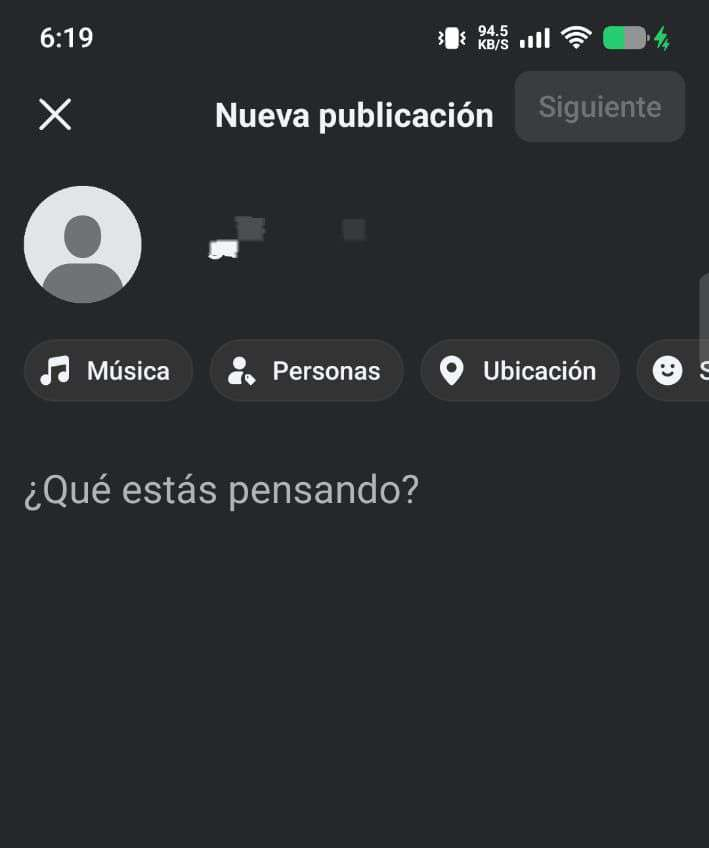
\includegraphics[width=\linewidth,height=4.05cm,keepaspectratio]{figuras/F2.png}\\{\scriptsize\textbf{F2.} Editor de publicación}\end{minipage}\hfill
\begin{minipage}[t]{0.31\linewidth}\centering
\includegraphics[width=\linewidth,height=4.05cm,keepaspectratio]{figuras/F3.png}\\{\scriptsize\textbf{F3.} Selector de reacciones}\end{minipage}
\begin{minipage}[t]{0.31\linewidth}\centering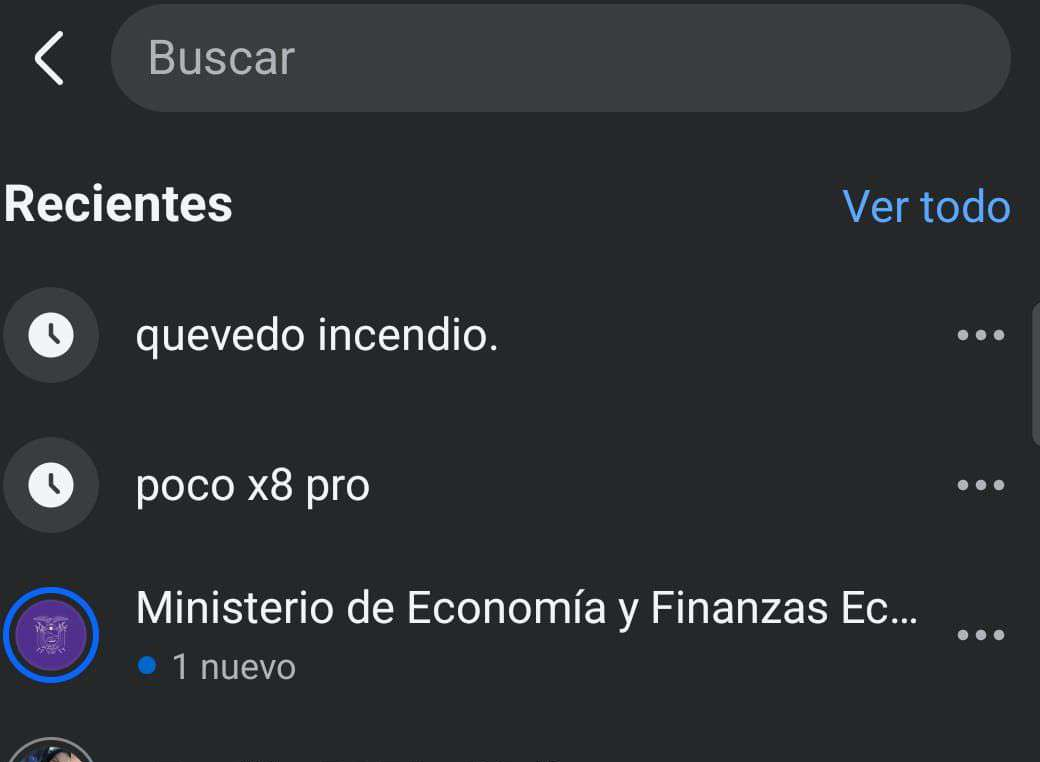
\includegraphics[width=\linewidth,height=4.05cm,keepaspectratio]{figuras/F4.png}\\{\scriptsize\textbf{F4.} Recientes en Buscar}\end{minipage}\hfill
\begin{minipage}[t]{0.31\linewidth}\centering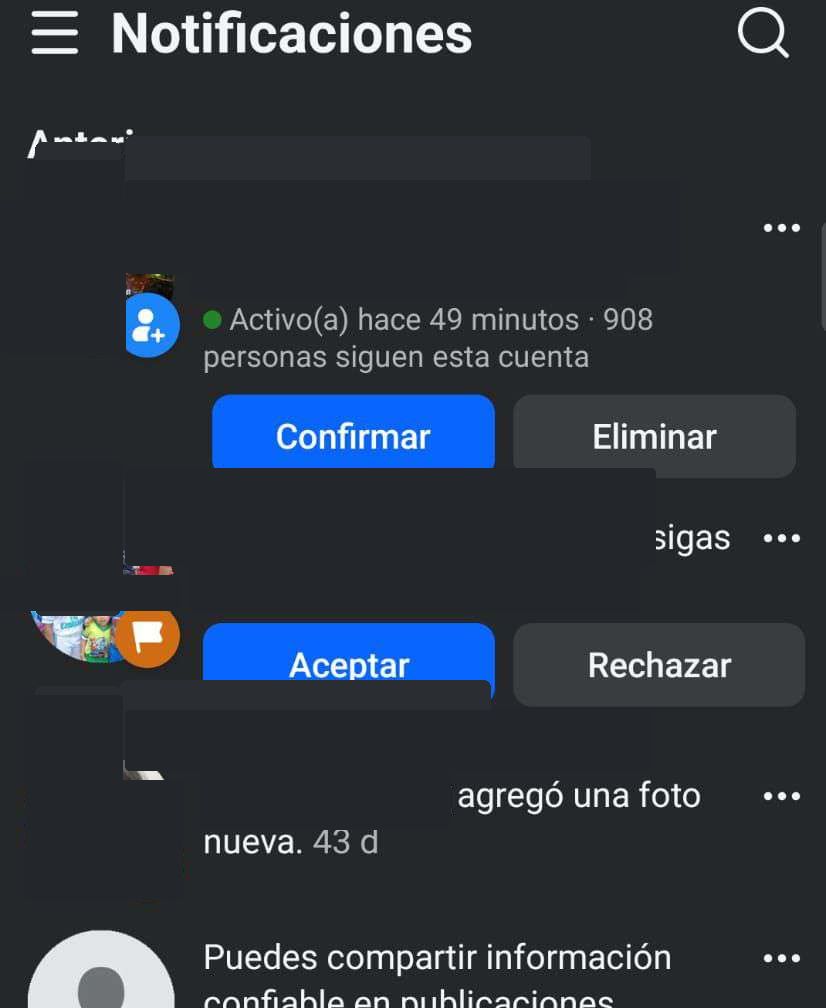
\includegraphics[width=\linewidth,height=4.05cm,keepaspectratio]{figuras/F5.png}\\{\scriptsize\textbf{F5.} Notificaciones}\end{minipage}\hfill
\begin{minipage}[t]{0.31\linewidth}\centering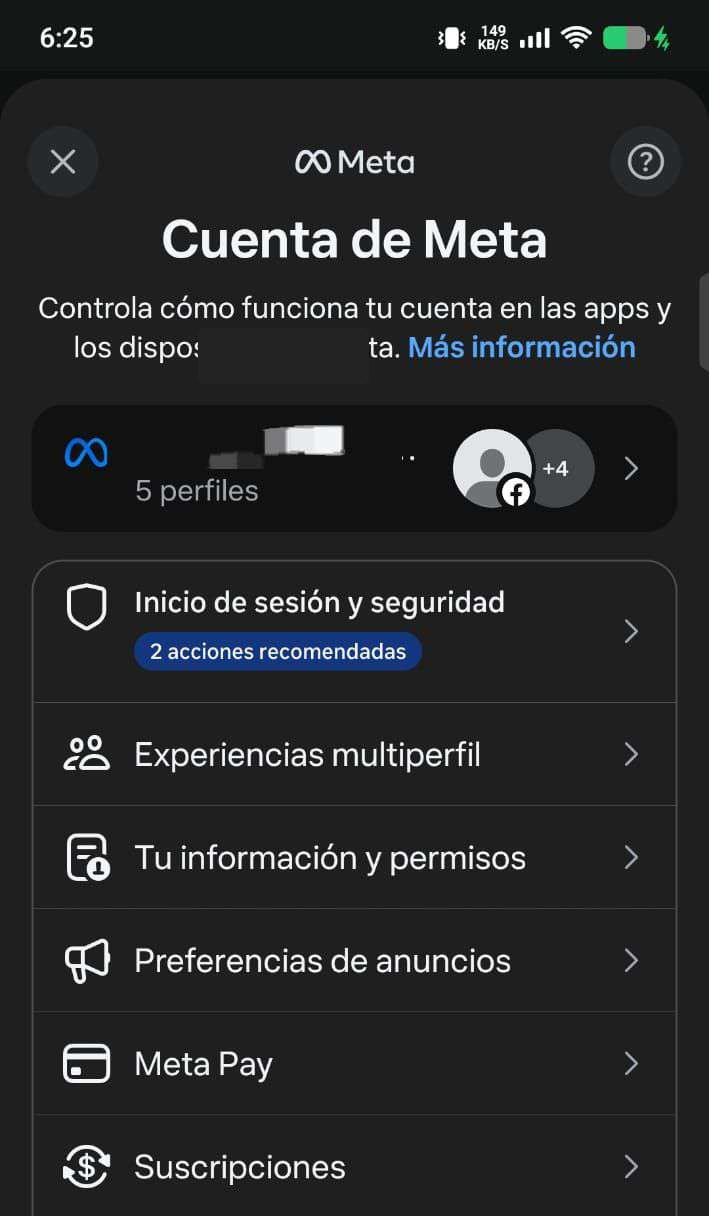
\includegraphics[width=\linewidth,height=4.05cm,keepaspectratio]{figuras/F6.png}\\{\scriptsize\textbf{F6.} Cuenta de Meta}\end{minipage}
\caption{Interfaz observada en Facebook móvil: paneles F1--F6. Elaboración a partir de capturas suministradas por la estudiante.}\label{fig:evidencias}\end{figure}
\seccion{7. Reflexión crítica}
Al analizar los requisitos de Facebook, una dificultad importante fue diferenciar la experiencia de uso cotidiano de una especificación formal conforme a ISO/IEC/IEEE 29148:2018. Expresiones como «rápido», «fácilmente» o «siempre» parecen claras en una conversación, pero no permiten establecer una prueba objetiva. La matriz de nueve características ayuda a identificar por qué esas expresiones deben reemplazarse por condiciones y resultados medibles. También fue necesario separar requisitos derivados de una misma pantalla: RF-05 plantea mostrar notificaciones; RI-07 se refiere a los botones de una solicitud; RH-10 propone un área táctil mínima y RC-14 define un criterio de ausencia de cierres inesperados. Aunque se relacionan con Notificaciones, no representan la misma obligación.

Otra dificultad es establecer métricas sin atribuir a Facebook resultados que no se han medido. Umbrales como tres segundos para mostrar la primera publicación, cuatro de cinco personas para localizar el buscador o cero cierres en treinta aperturas describen posibles criterios de aceptación, pero todavía necesitan comprobaciones. Las seis capturas aportadas permiten reconocer la interfaz, no demostrar el rendimiento, la seguridad ni los procesos internos de Meta. Por eso es relevante distinguir entre evidencia observada, requisito propuesto y prueba ejecutada; esa distinción evita confundir una especificación académica con una evaluación experimental del producto.
\seccion{8. Declaración de apoyo tecnológico y límites}
Se emplearon herramientas de inteligencia artificial como apoyo: ChatGPT (OpenAI, modelo GPT-6) y Gemini (Google, versión no consignada en el material recibido). Su intervención incluyó la preparación y edición de borradores del resumen, glosario, requisitos, tablas, reflexión y código LaTeX. Las seis capturas proceden de la estudiante; se compararon los nombres visibles de controles y pantallas con el contenido propuesto y se verificó la compilación de este archivo. Los umbrales son propuestas académicas, no resultados de pruebas. No se reportan entrevistas, mediciones de rendimiento ni auditorías de seguridad efectuadas.
\clearpage
\seccion{9. Protocolo de comprobación pendiente}
Los siguientes procedimientos proponen cómo evaluar los cinco requisitos de calidad. \textbf{No se han ejecutado}; por tanto, no se reportan tiempos, tasas de éxito ni resultados de seguridad. Los criterios se encuentran en la Tabla~\ref{tab:requisitos}.\par\smallskip
{\small
\begin{tabularx}{\linewidth}{@{}p{1.5cm}X@{}}\toprule
\textbf{ID}&\textbf{Procedimiento de prueba sugerido}\\\midrule
RC-11 & Estabilizar la conexión Wi-Fi (al menos 20 Mb/s), registrar el instante de entrada a Inicio y el momento en que aparece la primera tarjeta. Repetir veinte veces y contar cuántas cumplen el límite.\\[3pt]
RC-12 & Mantener una consulta en el historial, abrir Buscar veinte veces en las mismas condiciones de red y medir hasta visualizar Recientes; registrar la proporción dentro del umbral.\\[3pt]
RC-13 & Abrir Nueva publicación sin escribir texto, intentar avanzar veinte veces y anotar cualquier ocasión en que el control Siguiente deje continuar.\\[3pt]
RC-14 & Abrir Notificaciones treinta veces consecutivas en Samsung Android 16, documentando eventos de cierre inesperado durante el procedimiento.\\[3pt]
RC-15 & Cerrar sesión y realizar veinte intentos de acceso a «Tu información y permisos» de esa cuenta; comprobar si se exige nueva autenticación sin divulgar datos personales.\\\bottomrule
\end{tabularx}}\par
\smallskip
\textbf{Limitación del alcance:} no se dispone de código fuente de Facebook, entorno controlado de servidor ni representantes oficiales para validar requisitos de proceso. La validación definitiva requiere pruebas autorizadas y revisión por interesados.

\vspace{-9pt}
{\footnotesize\bibliographystyle{IEEEtran}\bibliography{referencias}}
\end{document}
